\begin{theorem}
  For every graph \(G\), 
  \[ \chi(G) \leq \Delta(G) + 1 \]
\end{theorem}

\begin{proof}
  If \(n=1\), then \(\chi(G) = 1 \leq 1+0 = 1 + \Delta(G)\). Now,
  assume that the claim satisfies for all graph with \(n-1\)
  vertices. Let \(G\) be a graph of \(n\) vertices. Let \(v\) be
  a vertex of \(G\). By the inductive hypothesis, we have
  \[
    \begin{aligned}
      \chi(G-v) &\leq 1 + \Delta(G-v) \\
                &\leq 1 + \Delta(G)
    \end{aligned}
  \]
  Hence, \(G-v\) can be colored with \(1+\Delta(G)\) colors. We
  then fix this coloring. Since there are at most \(\Delta(G)\)
  neighbors of \(v\), there will be an unused color for \(v\).
  Therefore, we need \(\leq 1+\Delta(G)\) to color \(G\).
\end{proof}

\section{Algorithm for Coloring}

There exists a greedy algorithm to solve the coloring problem.
Note that we will denote the colors by integers in set \(C\). The
full algorithm can be see in Algorithm \ref{alg:greedy-color}.
We can see that the running time is \(\mathcal{O}(n+m)\) since we
inspect every vertex once and we inspect each edge twice.

\begin{algorithm}
\caption{GreedyColor}
\label{alg:greedy-color}
\begin{algorithmic}
  \Input{Graph \(G\) of order \(n\)}
  \Output{Colored graph \(G\)}
  \State{\(\sigma \gets{}\) the order that the vertices will be
  processed}
  \For{\(i=1, 2, \ldots, n\)}
    \State{\(C_{N(\sigma_i)} \gets \text{colors used by neighbors
    of \(\sigma_i\)}\)}
    \State{\(\sigma_i \gets \min_{c \in \mathbb{N} \setminus
    C_{N(\sigma_i)} } c\)}
  \EndFor
\end{algorithmic}
\end{algorithm}

\section{Four Color Theorem}

\begin{conjecture}[Four Color Map Conjecture, 1852]
  No more than four colors are required to color the regions of
  any map so that no two adjacent regions have the same color.
\end{conjecture}

In order to \textit{proof} this conjecture, we need to transform
it into a more mathematical model. Notice that we can turn every
map into a planar graph by letting a vertex represent a country
and each country is adjacent to countries it shares a border
with. See example in Figure \ref{fig:map-and-dual}. Hence the 
study of coloring the map can be translated to the study of
coloring of the planar graph.

\begin{figure}[ht]
  \begin{center}
    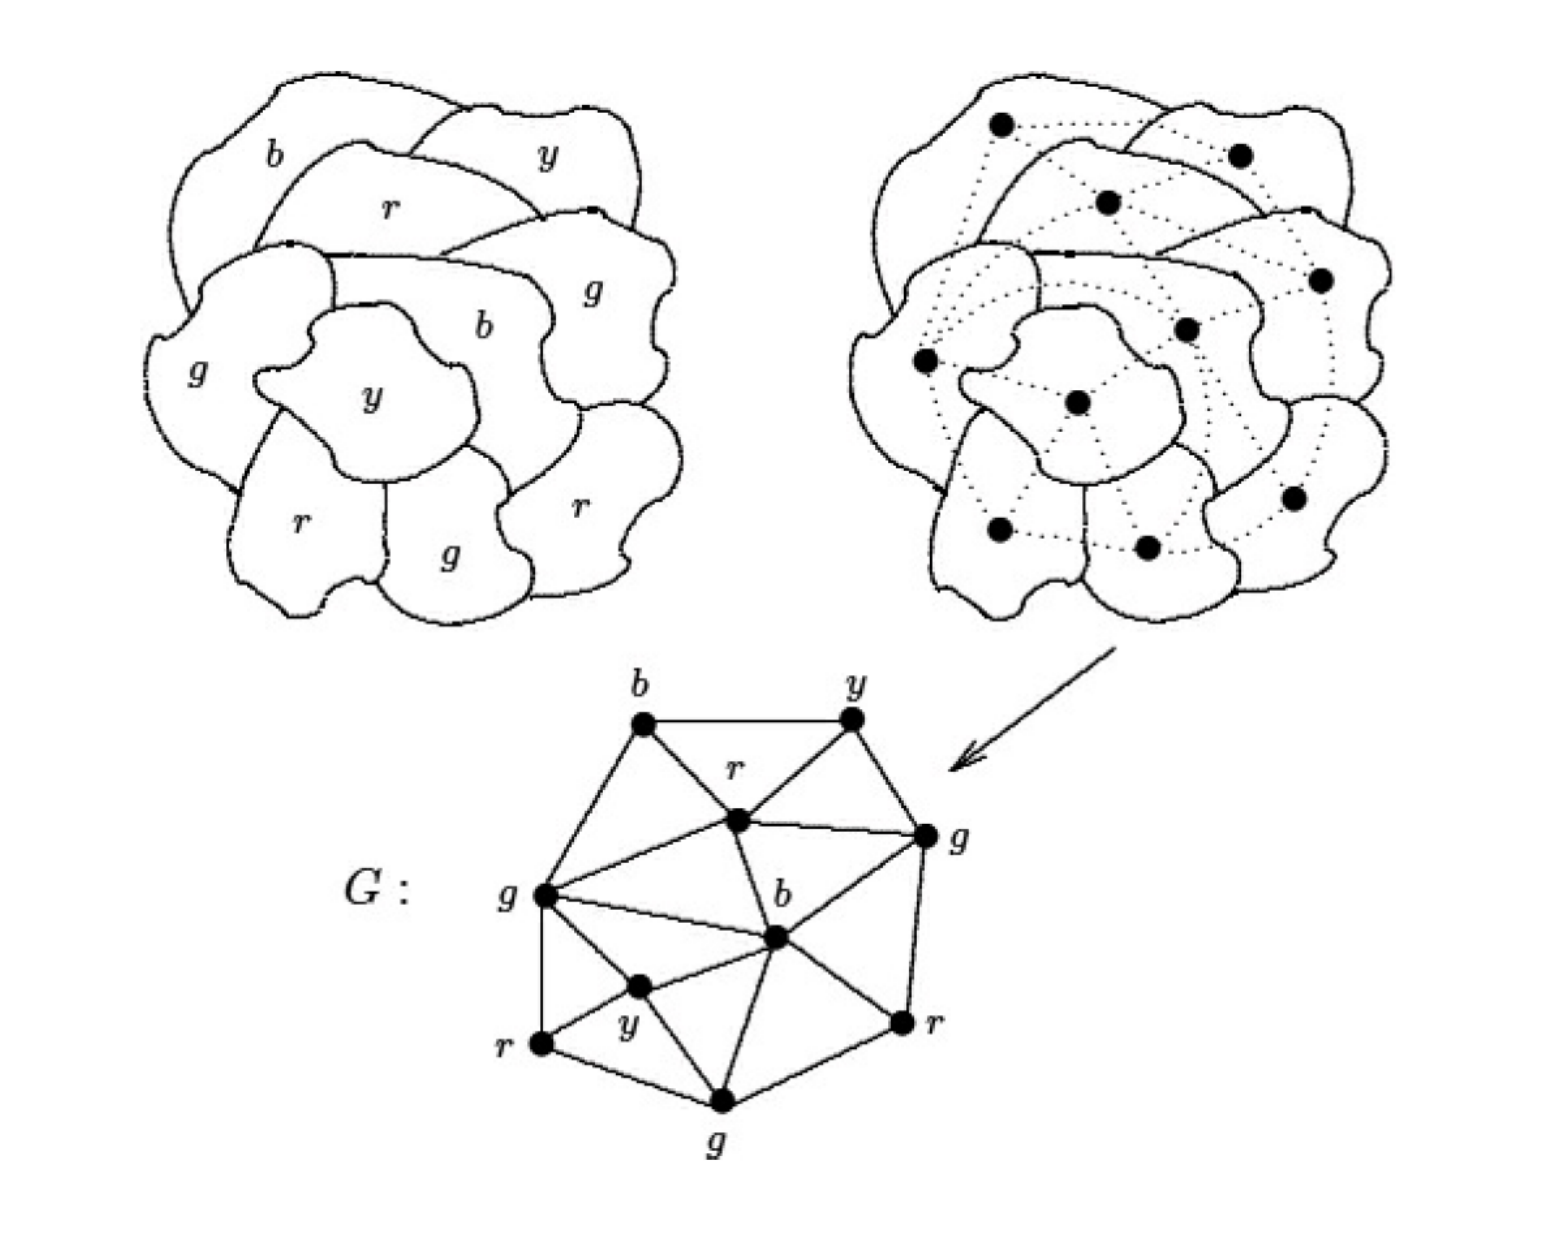
\includegraphics[width=0.69\textwidth]{figures/l15/map-and-dual}
  \end{center}
  \caption{A map and its dual}
  \label{fig:map-and-dual}
\end{figure}

\begin{distraction}
  \noindent\textbf{History of the Four Color Problem.}
  Evidently, this question originated not with map-makers but 
  with a mathematician. In 1852 Francis Guthrie (1831-1899), a
  recent graduate of University College London, observed that the 
  counties of England could be colored with four colors so that
  neighboring counties were colored differently. Francis Guthrie 
  found maps where three colors weren't enough but he felt that
  four colors were enough for all maps and he attempted to prove
  this. He showed his "proof" to his younger brother Frederick,
  who was taking a class at the time from the well-known Augustus
  De Morgan. Francis was not completely happy with the proof he 
  had given, however. With Francis' permission, Frederick showed 
  what Francis had written to De Morgan on October 23, 1852. De
  Morgan was pleased with this and felt it was new.

  De Morgan continued to be interested in it. Overall interest in
  this problem subsided during the next several years however.

  The proof initiated some controversial at the time as it is
  the very first computer assisted proof. In June 1976, Appel and
  Haken succeeded in constructing an unavoidable set of 1936
  reducible configurations, which was verified using 1200 hours
  of computer time on three computers. Appel and Haken announced
  their success to the world at the 1976 Summer Meeting of the
  American Mathematical Society and the Mathematical Association
  of America at the University of Toronto.

  In fact, a simpler solution (still computer assisted), employing
  an unavoidable set of 633 reducible configurations, was given in
  1993 by Neil Robertson, Daniel P. Sanders, Paul Seymour and 
  Robin Thomas.

  We will not prove the four color theorem during this class.
  But we will prove the six color theorem and the five color 
  theorem instead.
\end{distraction}

\begin{theorem}[The Four Color Theorem]
  The chromatic number of every planar graph is at most 4.
\end{theorem}

As mentioned in the history lesson above, there is still no
human-only proof for the Four Color Theorem. So, we will omit the
proof. We will, however, prove the Six Color Theorem.

\begin{theorem}
  Every planar graph is \(6\)-colorable.
\end{theorem}

\begin{proof}
  Recall that every planar graph contains a vertex with degree 5
  or less. We will prove our claim by induction on the number of
  vertices. When \(n=1\), the graph is 6-colorable since there is
  only one vertex. This will be the basis for our proof.
  We will now show the inductive case. 

  Assume that a graph of order \(n-1\) is 6-colorable. Let \(G\)
  be a planar graph of order \(n\) and \(v\) be a vertex such that
  \(\deg v \leq 5\). Consider \(G' = G-v\). Observe that \(G'\)
  is a planar graph of order \(n-1\). By the inductive hypothesis,
  \(G'\) is 6-colorable. Then, the neighborhood of \(v\) can be
  colored by at most 5 colors---leaving 1 unused color left for
  \(v\). Therefore, \(G\) is 6-colorable.   
\end{proof}

\begin{theorem}
  Every planar graph is 5-colorable.
\end{theorem}

\begin{proof}
  % We will use induction on the number of vertices. When \(n=1\),
  % the graph is 5-colorable. This will be the basis for our
  % inductive proof.

  % Let \(v\) be a vertex with \(\deg v \leq 5\) and \(G' = G-v\).
  % Assume also that \(G'\) is 5-colorable. If \(|N(v)| < 5\), then
  % we are done. Otherwise, suppose that neighbors of \(v\) are
  % \(N(v) = \{v_1, v_2, v_3, v_4, v_5\}\) and with correspondings
  % colors 1, 2, 3, 4, 5. We want to recolor \(\{v\} \cup N(v)\)
  % such that it is 5-colorable.

  % Consider the path starting with \(v_1\). There are a few cases.
  % \begin{enumerate}
  %   \item 
  %   \item There is a \(v_1-v_3\) path with coloring
  %     \(1-3-1-3-\cdots-1-3\). Then, there is no \(2-5-2-5\) path
  %     from \(v_2\) to \(v_5\) since \(v_2\) is enclosed in the
  %     \(1-3-\cdots-1-3\) path so there would have to be a vertex
  %     with color 1 or 3 in a \(v_2-v_5\) path somewhere. Then, we
  %     recolor \(v\) with 2 (or 5), recolor \(v_2\) (\(v_5\)) with
  %     1 or 3.
  % \end{enumerate}
  [Will rewrite later]
\end{proof}

